\documentclass[tikz,border=2pt]{standalone}
\usepackage[T1]{fontenc}\usepackage{helvet}\usepackage{amsmath}\usepackage{graphicx}
% shared TikZ styles for the three block diagrams (editable sources)
\usetikzlibrary{arrows.meta,positioning,fit,calc,backgrounds,shapes.geometric}
\definecolor{learn}{HTML}{6250D6}   % learned components
\definecolor{numer}{HTML}{2A78D6}   % numerical methods (Kalman lineage)
\definecolor{numerh}{HTML}{EB6834}  % numerical methods (Khalil lineage)
\definecolor{check}{HTML}{1D6B43}   % deterministic checks
\definecolor{ink}{HTML}{1B2430}
\definecolor{mut}{HTML}{5D6B7A}
\tikzset{
  every node/.style={font=\sffamily\scriptsize,text=ink,execute at begin node={\hyphenpenalty=10000 \exhyphenpenalty=10000 }},
  box/.style={draw=mut,rounded corners=1.5pt,line width=0.5pt,align=center,inner sep=3.5pt,fill=white,minimum height=6.5mm},
  learned/.style={box,draw=learn,dashed,line width=0.8pt,fill=learn!7},
  numeric/.style={box,draw=numer,line width=0.8pt,fill=numer!7},
  numerich/.style={box,draw=numerh,line width=0.8pt,fill=numerh!8},
  checkb/.style={box,draw=check,line width=0.8pt,double,double distance=0.6pt,fill=check!6},
  user/.style={box,fill=black!5},
  arr/.style={-{Stealth[length=4pt,width=3.4pt]},line width=0.5pt,draw=ink},
  darr/.style={arr,dashed},
  lab/.style={font=\sffamily\fontsize{6}{7}\selectfont,text=mut,align=center},
  onl/.style={lab,fill=white,inner sep=1.5pt},
  group/.style={draw=mut,dotted,line width=0.6pt,rounded corners=3pt,inner sep=5pt},
}

\tikzset{every node/.append style={font=\sffamily\footnotesize},
         lab/.style={font=\sffamily\fontsize{7}{8}\selectfont,text=mut,align=center},
         ctx/.style={box,dashed,fill=white},
         frame/.style={draw=mut,line width=0.5pt,inner sep=1.2pt,fill=white}}
% Portraits: portrait_kalman.jpg and portrait_khalil.jpg (4:3 crops of the supplied illustrations) next to this file;
% the name is printed under each portrait.  Without the files, a name card takes their place.
\newcommand{\portrait}[3]{\IfFileExists{#1.jpg}%
  {\begin{tabular}{@{}c@{}}\includegraphics[width=2.7cm,height=2.05cm,keepaspectratio]{#1.jpg}\\[-0.5pt]
     {\fontsize{7}{8}\selectfont\textbf{#2}\ifx\relax#3\relax\else\ (#3)\fi}\end{tabular}}%
  {\parbox[c][2.05cm][c]{2.7cm}{\centering\textbf{#2}\\[2pt]{\fontsize{7}{8}\selectfont #3}}}}
\begin{document}
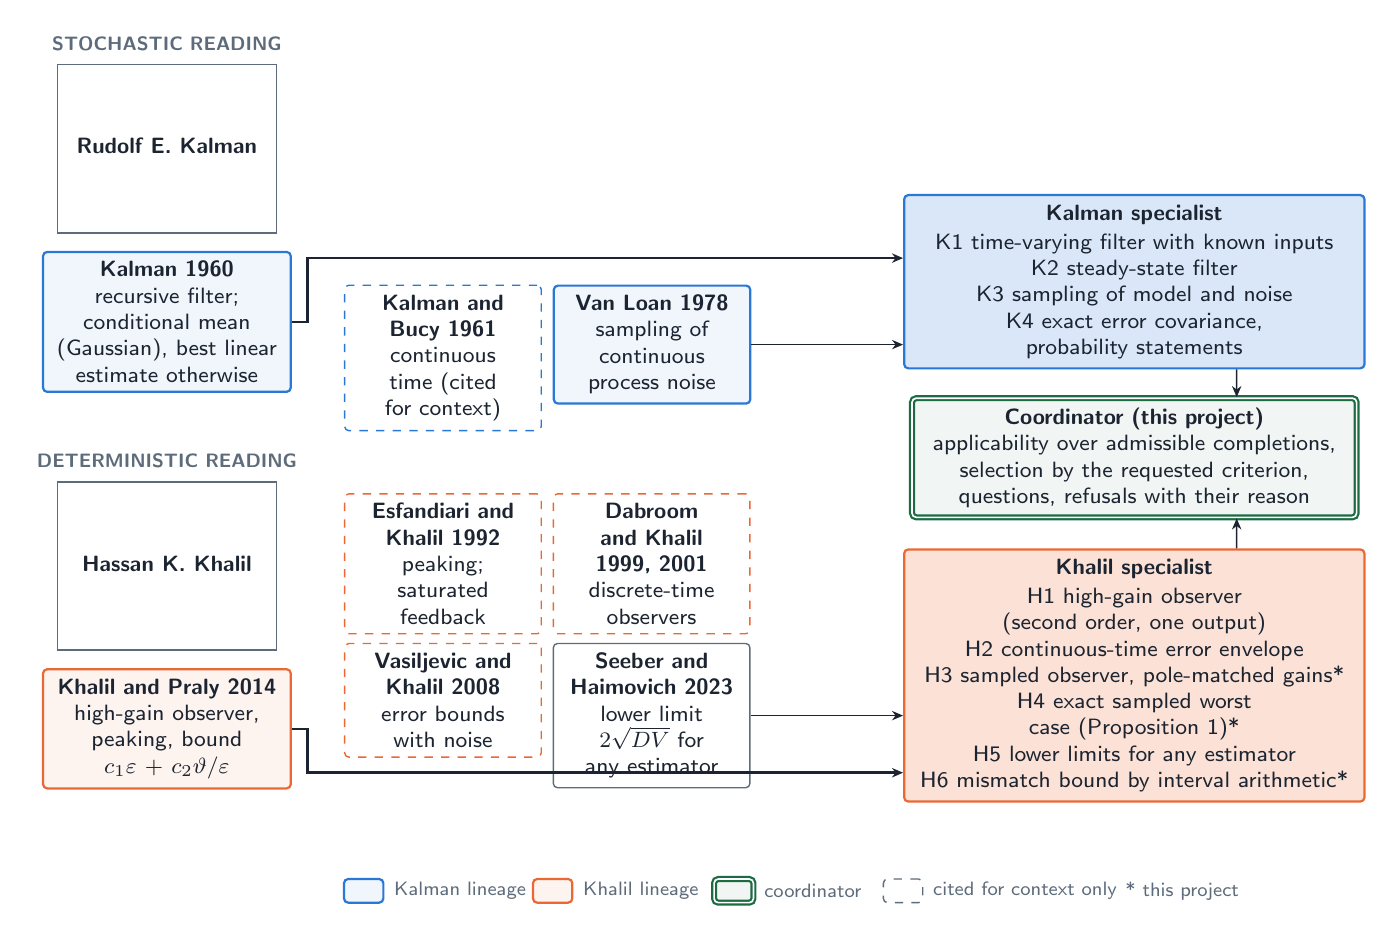
\begin{tikzpicture}[x=1cm,y=1cm,node distance=3mm]
% ---------------- Kalman: portrait above the method, method to the specialist ----------------
\node[frame,anchor=north west] (pk) at (0,7.75) {\portrait{portrait_kalman}{Rudolf E. Kalman}{}};
\node[numeric,text width=2.9cm,anchor=north] (k60) at ($(pk.south)+(0,-0.22)$) {\textbf{Kalman 1960}\\ recursive filter; conditional mean (Gaussian), best linear estimate otherwise};
\node[ctx,draw=numer,text width=2.25cm,anchor=north west] (kb) at (3.65,4.95) {\textbf{Kalman and Bucy 1961}\\ continuous time (cited for context)};
\node[numeric,text width=2.25cm,anchor=north west] (vl) at (6.3,4.95) {\textbf{Van Loan 1978}\\ sampling of continuous process noise};
\node[numeric,fill=numer!18,text width=5.6cm,anchor=north west] (K) at (10.75,6.1) {\textbf{Kalman specialist}\\[1pt]
  K1 time-varying filter with known inputs\\ K2 steady-state filter\\ K3 sampling of model and noise\\ K4 exact error covariance, probability statements};
\coordinate (kin) at ($(K.west)+(0,0.3)$);
\draw[arr,line width=0.9pt] (k60.east) -- ++(0.2,0) |- (kin);
\draw[arr] (vl.east) -- (vl.east -| K.west);
\node[lab,anchor=south] at ($(pk.north)+(0,0.05)$) {\textbf{STOCHASTIC READING}};
% ---------------- coordinator ----------------
\node[checkb,text width=5.4cm,anchor=west] (C) at (10.85,2.75) {\textbf{Coordinator (this project)}\\ applicability over admissible completions,\\ selection by the requested criterion,\\ questions, refusals with their reason};
\draw[arr] ($(K.south)+(1.3,0)$) -- ($(C.north)+(1.3,0)$);
% ---------------- Khalil: portrait above the method, method to the specialist ----------------
\node[frame,anchor=north west] (ph) at (0,2.45) {\portrait{portrait_khalil}{Hassan K. Khalil}{}};
\node[numerich,text width=2.9cm,anchor=north] (kp) at ($(ph.south)+(0,-0.22)$) {\textbf{Khalil and Praly 2014}\\ high-gain observer, peaking, bound $c_1\varepsilon + c_2\vartheta/\varepsilon$};
\node[ctx,draw=numerh,text width=2.25cm,anchor=north west] (ek) at (3.65,2.3) {\textbf{Esfandiari and Khalil 1992}\\ peaking; saturated feedback};
\node[ctx,draw=numerh,text width=2.25cm,anchor=north west] (dk) at (6.3,2.3) {\textbf{Dabroom and Khalil 1999, 2001}\\ discrete-time observers};
\node[ctx,draw=numerh,text width=2.25cm,anchor=north west] (vk) at (3.65,0.4) {\textbf{Vasiljevic and Khalil 2008}\\ error bounds with noise};
\node[box,text width=2.25cm,anchor=north west] (sh) at (6.3,0.4) {\textbf{Seeber and Haimovich 2023}\\ lower limit $2\sqrt{DV}$ for any estimator};
\node[numerich,fill=numerh!20,text width=5.6cm,anchor=north west] (H) at (10.75,1.6) {\textbf{Khalil specialist}\\[1pt]
  H1 high-gain observer (second order, one output)\\ H2 continuous-time error envelope\\ H3 sampled observer, pole-matched gains*\\
  H4 exact sampled worst case (Proposition~1)*\\ H5 lower limits for any estimator\\ H6 mismatch bound by interval arithmetic*};
\coordinate (hin) at (10.75,-1.25);
\draw[arr,line width=0.9pt] (kp.east) -- ++(0.2,0) |- (hin);
\draw[arr] (sh.east) -- (H.west |- sh.east);
\draw[arr] ($(H.north)+(1.3,0)$) -- ($(C.south)+(1.3,0)$);
\node[lab,anchor=south] at ($(ph.north)+(0,0.05)$) {\textbf{DETERMINISTIC READING}};
% legend
\node[numeric,minimum width=5mm,minimum height=3mm,inner sep=0pt] (l1) at (3.9,-2.75) {}; \node[lab,anchor=west] at (l1.east) {Kalman lineage};
\node[numerich,minimum width=5mm,minimum height=3mm,inner sep=0pt] (l2) at (6.3,-2.75) {}; \node[lab,anchor=west] at (l2.east) {Khalil lineage};
\node[checkb,minimum width=5mm,minimum height=3mm,inner sep=0pt] (l3) at (8.6,-2.75) {}; \node[lab,anchor=west] at (l3.east) {coordinator};
\node[ctx,minimum width=5mm,minimum height=3mm,inner sep=0pt] (l4) at (10.75,-2.75) {}; \node[lab,anchor=west] at (l4.east) {cited for context only};
\node[lab,anchor=west] at (13.45,-2.75) {* this project};
\end{tikzpicture}
\end{document}
